% !TeX program = pdflatex
\documentclass[14pt,a4paper]{extreport}

\usepackage[a4paper,left=30mm,right=10mm,top=20mm,bottom=20mm]{geometry}
\usepackage[T2A]{fontenc}
\usepackage[utf8]{inputenc}
\usepackage[main=russian,english]{babel}

\usepackage{setspace}
\renewcommand{\baselinestretch}{1.2}
\usepackage{indentfirst}
\setlength{\parindent}{1.25cm}

\usepackage{graphicx}
\usepackage{float}
\usepackage{booktabs}
\usepackage{tabularx}
\usepackage{array}
\usepackage{caption}
\usepackage{hyperref}
\usepackage{titlesec}
\usepackage{tocloft}
\usepackage{csquotes}
\usepackage{pgfplots}
\usepackage{svg}
\usepackage[backend=biber,sorting=none]{biblatex}
\addbibresource{references.bib}

\pgfplotsset{compat=1.18}

\hypersetup{
    colorlinks=true,
    linkcolor=black,
    urlcolor=blue,
    citecolor=black
}

\addto\captionsrussian{%
  \renewcommand{\chaptername}{ГЛАВА}%
  \renewcommand{\chaptertitlename}{ГЛАВА}%
  \renewcommand{\figurename}{Рисунок}%
  \renewcommand{\tablename}{Таблица}%
  \renewcommand{\contentsname}{\makebox[\textwidth][c]{ОГЛАВЛЕНИЕ}}%
}
\captionsetup[figure]{labelsep=space,justification=centering}
\captionsetup[table]{labelsep=space,justification=centering}

\titleformat{\chapter}[display]
  {\centering\Large\bfseries}
  {\chaptertitlename\ \thechapter}
  {10pt}
  {\Large}
\titlespacing*{\chapter}{5pt}{-20pt}{30pt}

\titleformat{\section}[block]
  {\large\bfseries}
  {\thesection\ }{0pt}{}

\renewcommand{\cftchapfont}{\bfseries}
\renewcommand{\cftchappagefont}{\bfseries}
\renewcommand{\cfttoctitlefont}{\large\bfseries}
\setlength{\cftbeforechapskip}{0.3em}
\setlength{\cftbeforetoctitleskip}{0pt}
\setlength{\cftaftertoctitleskip}{0.5\baselineskip}

\begin{document}
\selectlanguage{russian}

\setcounter{page}{1}
\setstretch{1.0}
\thispagestyle{empty}
\newgeometry{left=0mm,top=20mm,right=0mm,bottom=20mm}
\begin{center}
\bfseries
\vspace{4cm}
{
\setstretch{0.9}
\mbox{МИНИСТЕРСТВО~ОБРАЗОВАНИЯ~РЕСПУБЛИКИ~БЕЛАРУСЬ} \\~\\
\mbox{БЕЛОРУССКИЙ~ГОСУДАРСТВЕННЫЙ~УНИВЕРСИТЕТ} \\~\\
\mbox{МЕХАНИКО-МАТЕМАТИЧЕСКИЙ~ФАКУЛЬТЕТ} \\~\\
\mbox{Кафедра~дифференциальных~уравнений~и~системного~анализа} \\~\\
}
\vspace{4cm}
\mbox{ОБУЧЕНИЕ С ПОДКРЕПЛЕНИЕМ ДЛЯ ИГРЫ <<ЗМЕЙКА>>}\\
\vspace{1cm}
\rmfamily Курсовая работа
\vspace{3cm}
\end{center}

\begin{tabular}{ll}
\hspace{10.5cm}
&Полегина Александра Дмитриевича\\~\\
&студента 3-го курса\\
&специальности 6-05-0533-08\\
&<<Компьютерная математика\\
&и системный анализ>>\\~\\
&Научный руководитель:\\
&кандидат физ.-мат. наук,\\
&доцент С.~Г.~Красовский
\end{tabular}
\vspace{4cm}
\begin{center}
    Минск, 2026
\end{center}
\clearpage
\restoregeometry
\setstretch{1.2}

\tableofcontents
\clearpage

\chapter*{\large ВВЕДЕНИЕ}
\addcontentsline{toc}{chapter}{ВВЕДЕНИЕ}

Игра <<Змейка>> хорошо подходит для изучения обучения с подкреплением. В ней каждое действие сразу влияет на дальнейшую ситуацию на поле и на итоговый счёт. Поэтому на такой задаче удобно разбирать, как задаются состояния, действия и награды, и как агент постепенно учится принимать более удачные решения.

Тема работы актуальна потому, что обучение с подкреплением позволяет строить агентов, которые учатся на собственном опыте, а не по заранее прописанным правилам для каждой ситуации. Даже на сравнительно простой игре можно проследить все основные этапы разработки такой системы: создание среды, выбор признаков состояния, настройку награды, обучение и проверку результатов.

Цель курсовой работы --- разработать игру <<Змейка>> на языке Python, реализовать алгоритм обучения с подкреплением для управления агентом и оценить, насколько хорошо он обучается.

Для достижения этой цели были поставлены следующие задачи:
\begin{itemize}
    \item изучить основные идеи обучения с подкреплением и алгоритма Q-learning;
    \item разобрать требования к игровой среде и реализовать логику игры <<Змейка>>;
    \item задать пространство состояний, множество действий и функцию награды;
    \item реализовать агента и процесс накопления Q-таблицы;
    \item провести вычислительные эксперименты и оценить, как меняется качество игры во время обучения;
    \item подготовить таблицы, графики и изображения, которые объясняют устройство программы и поведение агента.
\end{itemize}

Объект исследования --- программная игра <<Змейка>>. Предмет исследования --- методы обучения с подкреплением для выбора действий в дискретной игровой среде. В работе используются методы объектно-ориентированного программирования, имитационного моделирования и вычислительного эксперимента.

\chapter{АНАЛИЗ ЗАДАЧИ И ПОДХОДОВ К ЕЁ РЕШЕНИЮ}

\section{Постановка задачи управления в игре <<Змейка>>}

В этой задаче нужно построить агента, который управляет змейкой на дискретном поле и старается набрать как можно больше очков. На каждом шаге агент выбирает действие по текущему состоянию игры, после чего среда возвращает новое состояние и награду. Поэтому задачу удобно рассматривать как последовательное принятие решений.

Особенность игры в том, что хороший ход не всегда даёт пользу сразу. Действие может выглядеть безопасным сейчас, но через несколько шагов привести либо к пище, либо к столкновению. Из-за этого агенту нужно учитывать не только ближайшую ситуацию, но и накопленный опыт.

\section{Особенности обучения с подкреплением для дискретной среды}

Обучение с подкреплением подходит для задач, где агент сам ищет удачную стратегию, взаимодействуя со средой и получая награды за свои действия. В отличие от обучения с учителем, здесь нет набора правильных ответов. Агент учится на том, к чему приводят его решения.

На шаге $t$ агент видит состояние $s_t$, выбирает действие $a_t$, получает награду $r_t$ и переходит в состояние $s_{t+1}$. Для игры <<Змейка>> такой подход удобен, потому что:
\begin{itemize}
    \item игра имеет дискретную структуру;
    \item число действий невелико;
    \item результат легко оценивать по счёту;
    \item поведение агента можно наглядно показать на экране.
\end{itemize}

Поэтому <<Змейка>> хорошо подходит для демонстрации базовых идей reinforcement learning на реальном проекте.

\section{Сравнение возможных подходов к решению}

Управлять змейкой можно по-разному. Самый простой вариант --- набор правил и эвристик. В этом случае разработчик заранее прописывает, как агент должен реагировать на опасность и как двигаться к пище. Такой подход легко начать, но он плохо переносится на более сложные игровые ситуации.

Другой вариант --- использовать алгоритмы поиска пути. Они могут строить маршрут к цели, но требуют отдельного планирования и хуже показывают сам процесс обучения на опыте.

Третий вариант --- методы обучения с подкреплением, например табличный Q-learning или более сложные нейросетевые методы, такие как DQN. В нашем проекте состояние уже сведено к компактному набору признаков, поэтому можно применять табличный метод без лишнего усложнения.

\begin{table}[H]
    \centering
    \caption{Сравнение подходов к управлению змейкой}
    \begin{tabularx}{\textwidth}{>{\raggedright\arraybackslash}p{0.22\textwidth} >{\raggedright\arraybackslash}p{0.24\textwidth} X}
        \toprule
        Подход & Преимущества & Ограничения \\
        \midrule
        Правила и эвристики & Простая реализация, предсказуемое поведение & Сложно покрыть все игровые ситуации, слабая адаптивность \\
        Поиск траектории & Явный контроль маршрута, хорош для детерминированных сценариев & Требует дополнительного планирования на каждом шаге, хуже отражает накопление опыта \\
        Табличный Q-learning & Интерпретируемость, простота обновления, естественная связь с дискретной средой & Ограниченная масштабируемость при росте пространства состояний \\
        DQN и другие глубокие методы & Хорошо работают на более сложных наблюдениях и больших пространствах состояний & Требуют больше данных, вычислений и настройки \\
        \bottomrule
    \end{tabularx}
\end{table}

\section{Обоснование выбора табличного Q-learning}

В этой работе выбран табличный Q-learning. На это есть две основные причины. Во-первых, он хорошо подходит для учебного проекта, потому что его легко объяснять и анализировать. Во-вторых, в проекте используется вектор состояния из 11 бинарных признаков, а значит Q-значения ещё можно хранить в таблице.

Такой выбор даёт хороший баланс между простотой и пользой. С одной стороны, метод не перегружает проект лишней сложностью. С другой стороны, он позволяет получить реальный обучаемый агент и показать, как меняется его поведение по мере накопления опыта.

\chapter{ПРОЕКТИРОВАНИЕ ИГРОВОЙ СРЕДЫ И ОБУЧАЮЩЕГО АГЕНТА}

\section{Требования к игровой среде}

Среда должна решать сразу две задачи. С одной стороны, она должна правильно реализовывать саму игру: движение змейки, появление пищи, рост длины и завершение партии при столкновении. С другой стороны, она должна быть удобной для обучения агента: возвращать состояние, принимать действие и выдавать численную награду.

В проекте используется поле размером $20 \times 20$ клеток. Змейка начинает движение из центра поля и сначала направлена вправо. Такое начальное положение удобно, потому что оно симметрично и не даёт преимущества какой-то одной стороне поля.

\begin{table}[H]
    \centering
    \caption{Основные параметры игровой среды и обучения}
    \begin{tabularx}{\textwidth}{>{\raggedright\arraybackslash}p{0.3\textwidth} >{\raggedright\arraybackslash}p{0.18\textwidth} X}
        \toprule
        Параметр & Значение & Назначение \\
        \midrule
        Размер поля & $20 \times 20$ & Количество клеток по горизонтали и вертикали \\
        Размер клетки & 24 px & Масштаб визуализации в окне Pygame \\
        FOOD\_REWARD & 10.0 & Награда за поедание пищи \\
        COLLISION\_PENALTY & -10.0 & Штраф за столкновение \\
        STEP\_PENALTY & -0.1 & Небольшой штраф за каждый ход \\
        ALPHA & 0.1 & Скорость обновления Q-оценок \\
        GAMMA & 0.9 & Учёт будущих вознаграждений \\
        EPSILON & 1.0 & Начальная интенсивность исследования \\
        EPSILON\_DECAY & 0.995 & Множитель снижения $\varepsilon$ \\
        EPSILON\_MIN & 0.05 & Нижняя граница $\varepsilon$ \\
        TRAIN\_EPISODES & 300 & Базовое число эпизодов обучения \\
        \bottomrule
    \end{tabularx}
\end{table}

\section{Формирование пространства состояний}

Одним из главных решений в проекте стал выбор состояния агента. Если хранить все координаты змейки и еды, число состояний быстро станет слишком большим. Поэтому в работе используется более компактный вариант --- вектор из 11 бинарных признаков.

В этот вектор входят признаки опасности при движении прямо, влево и вправо, текущее направление змейки и положение пищи относительно головы. Такой набор даёт агенту ту информацию, которая действительно нужна для выбора следующего хода, и при этом не делает модель слишком сложной.

Такой подход важен не только для удобства реализации, но и для самой логики обучения. Агенту не обязательно знать полную геометрию поля в каждый момент времени, если для принятия ближайшего решения ему достаточно понимать три вещи: есть ли опасность рядом, куда он сейчас движется и с какой стороны находится цель. За счёт этого состояние получается компактным и хорошо подходит для табличного Q-learning.

Ещё одно достоинство такого описания состоит в том, что оно делает поведение агента более обобщаемым. Разные игровые ситуации, которые с точки зрения координат выглядят по-разному, могут совпадать по смыслу: например, во всех них еда находится справа, а впереди есть опасность. В табличном методе это особенно полезно, потому что позволяет использовать один и тот же набор оценок для типовых игровых шаблонов.

\begin{table}[H]
    \centering
    \caption{Состав вектора состояния среды}
    \begin{tabularx}{\textwidth}{>{\centering\arraybackslash}p{0.08\textwidth} >{\raggedright\arraybackslash}p{0.26\textwidth} X}
        \toprule
        № & Признак & Смысл \\
        \midrule
        1 & danger\_straight & Столкновение при движении прямо \\
        2 & danger\_left & Столкновение при повороте влево \\
        3 & danger\_right & Столкновение при повороте вправо \\
        4 & dir\_up & Текущая ориентация вверх \\
        5 & dir\_down & Текущая ориентация вниз \\
        6 & dir\_left & Текущая ориентация влево \\
        7 & dir\_right & Текущая ориентация вправо \\
        8 & food\_left & Пища расположена левее головы \\
        9 & food\_right & Пища расположена правее головы \\
        10 & food\_up & Пища расположена выше головы \\
        11 & food\_down & Пища расположена ниже головы \\
        \bottomrule
    \end{tabularx}
\end{table}

\section{Множество действий и проектирование функции награды}

Вместо абсолютных направлений в проекте используются относительные действия: идти прямо, повернуть влево и повернуть вправо. Это упрощает обучение, потому что агент выбирает действие относительно своего текущего движения, а не относительно экрана.

Награда построена так, чтобы агенту было выгодно искать пищу и избегать бесполезных ходов. За поедание пищи он получает 10.0, за столкновение --- штраф -10.0, а за обычный шаг --- небольшой штраф -0.1. За счёт этого агент учится не просто долго жить, а двигаться к цели.

Выбор относительных действий особенно важен с точки зрения обучения. Если бы агент использовал абсолютные команды вроде <<вверх>>, <<вниз>>, <<влево>> и <<вправо>>, ему пришлось бы отдельно учиться похожим ситуациям для разных текущих направлений движения. Относительная схема уменьшает эту избыточность: действие <<повернуть влево>> имеет один и тот же смысл независимо от того, куда змейка была направлена до этого. Это делает пространство действий меньше и помогает агенту быстрее накапливать полезный опыт.

Функция награды тоже играет ключевую роль. Положительная награда за пищу даёт агенту явную цель. Штраф за столкновение показывает, какие ситуации являются критически плохими. Небольшой штраф за обычный шаг нужен для того, чтобы агент не выбирал бесконечное безопасное движение по кругу, которое не приводит к росту счёта. Иначе в задаче могла бы появиться стратегия, при которой агент долго избегает смерти, но почти не решает основную задачу.

С точки зрения проектирования это означает, что награда задаёт само понятие <<хорошего поведения>>. В данной работе хорошей считается стратегия, которая одновременно избегает столкновений, движется к пище и не тратит слишком много лишних шагов. Именно такой баланс и был заложен в систему вознаграждений.

\section{Архитектура программной системы}

Программа разбита на несколько модулей. Файл \texttt{game.py} отвечает за игровую механику, \texttt{env.py} превращает игру в среду для обучения, \texttt{agent.py} содержит Q-learning агента, \texttt{train.py} управляет обучением, \texttt{render.py} отвечает за визуализацию, а \texttt{main.py} запускает нужный режим работы.

\begin{figure}[H]
    \centering
    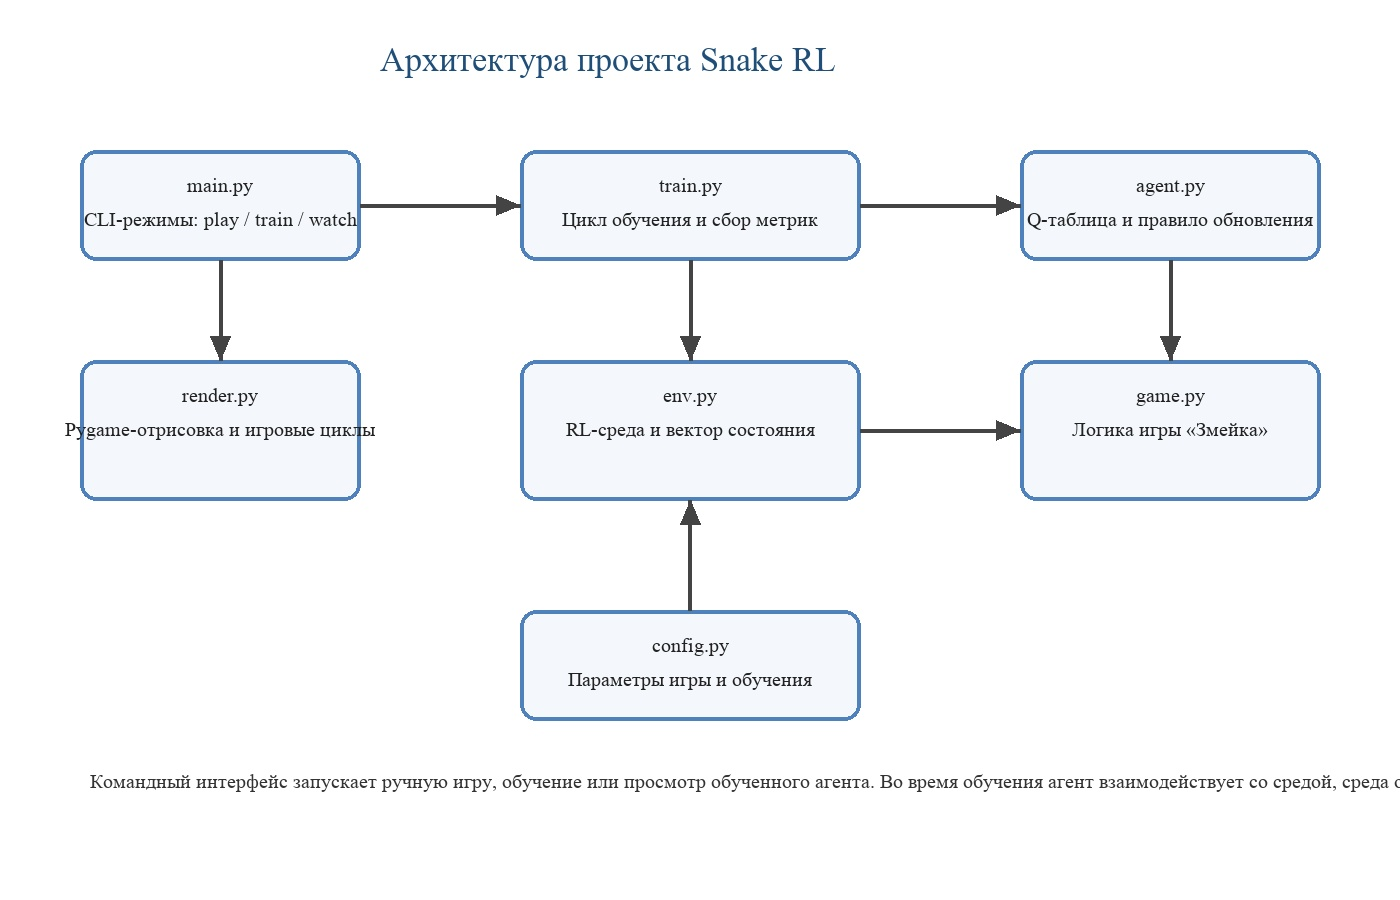
\includegraphics[width=0.92\textwidth]{images/architecture.jpg}
    \caption{Структурная схема взаимодействия модулей проекта}
\end{figure}

Такое разбиение делает проект более понятным и удобным для доработки. Игровую логику, обучение и интерфейс можно рассматривать как отдельные части системы.

Кроме того, такая архитектура удобна и для анализа результатов. Если агент обучается плохо, можно отдельно проверять, правильно ли работает игровая логика, корректно ли формируется состояние, верно ли считается награда и не ошибается ли модуль выбора действия. Это особенно важно в учебном проекте, где цель состоит не только в получении работающей программы, но и в понимании того, как взаимодействуют все её части.

\chapter{РЕАЛИЗАЦИЯ ПРОГРАММНОЙ СИСТЕМЫ}

\section{Реализация логики игры}

Базовый класс \texttt{SnakeGame} отвечает за основную механику игры. В нём реализованы положение головы и тела змейки, проверка столкновений, рост длины после поедания пищи и выбор свободной клетки для новой еды.

Также в игре есть защита от мгновенного разворота на 180 градусов. Это соответствует обычным правилам <<Змейки>> и убирает некорректные переходы между состояниями.

Такое разделение полезно тем, что игровая логика остаётся независимой от обучения. Игра умеет корректно работать сама по себе: обновлять положение объектов, проверять конец партии и поддерживать состояние поля. Благодаря этому один и тот же игровой движок можно использовать и для ручного режима, и для обучения, и для наблюдения за уже обученным агентом.

\section{Реализация RL-среды и Q-learning агента}

Среда переводит игровую механику в форму, удобную для обучения. По текущему положению змейки строится вектор состояния, затем принимается одно из трёх действий, после чего среда возвращает награду, новое состояние и признак завершения эпизода.

Класс \texttt{QLearningAgent} хранит Q-таблицу в виде словаря. Ключом служит кортеж признаков состояния, а значением --- список оценок для трёх действий. Если состояние встречается впервые, для него создаётся набор нулевых оценок.

Выбор действия строится по $\varepsilon$-жадному правилу: иногда агент делает случайный ход, а иногда выбирает лучший из уже известных. После каждого шага вызывается функция \texttt{update}, которая обновляет Q-значение для пары <<состояние --- действие>>.

Если рассмотреть один эпизод обучения по шагам, то процесс выглядит так. Сначала среда возвращает текущее состояние. Затем агент по этому состоянию выбирает действие. После выполнения действия игра переходит в новую конфигурацию, а среда вычисляет награду. Далее агент получает новое состояние и обновляет соответствующее значение в Q-таблице. Такой цикл повторяется до тех пор, пока змейка не столкнётся с препятствием или не завершится текущая партия.

Преимущество такой схемы в том, что она хорошо согласуется с формальной моделью reinforcement learning. Каждый шаг обучения можно описать как переход из одного состояния в другое с фиксированным действием и численной наградой. Это делает программу не просто игровой реализацией, а полноценной учебной RL-средой.

\section{Реализация интерфейса и режимов работы программы}

Визуальная часть сделана на библиотеке \texttt{pygame}. Программа рисует поле, еду, змейку, строку состояния и окно завершения игры. Также есть ручной режим и режим наблюдения за уже обученным агентом \cite{matthes2023python,pygame_docs}.

\begin{figure}[H]
    \centering
    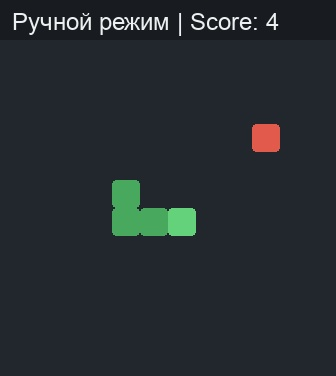
\includegraphics[width=0.42\textwidth]{images/manual_game.jpg}
    \caption{Интерфейс программы в режиме ручной игры}
\end{figure}

\begin{figure}[H]
    \centering
    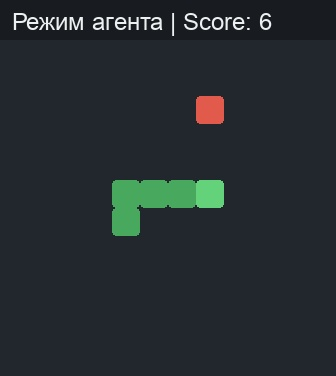
\includegraphics[width=0.42\textwidth]{images/agent_mode.jpg}
    \caption{Интерфейс программы в режиме наблюдения за агентом}
\end{figure}

\begin{figure}[H]
    \centering
    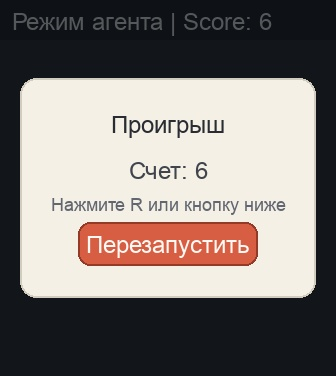
\includegraphics[width=0.42\textwidth]{images/game_over_modal.jpg}
    \caption{Модальное окно завершения партии и перезапуска}
\end{figure}

\section{Сохранение обученной политики и структура модулей}

После обучения таблица сохраняется в файл \texttt{artifacts/q\_table.pkl}. Благодаря этому можно запускать агента в режиме \texttt{watch} без повторного обучения. Это удобно и для экспериментов, и для демонстрации работы программы.

Практическая ценность сохранения Q-таблицы состоит в том, что обучение и демонстрация результатов становятся независимыми друг от друга. Не нужно каждый раз заново запускать длинную процедуру обучения, чтобы показать поведение агента. Можно один раз получить таблицу, а затем использовать её для серии визуальных запусков, сравнения поведения в разных ситуациях и подготовки иллюстраций для отчёта.

С точки зрения структуры проекта это решение также полезно тем, что отделяет этап накопления опыта от этапа использования уже готовой стратегии. Такая схема особенно удобна для курсовой работы: она позволяет сначала описать процесс обучения как вычислительный эксперимент, а затем отдельно показать практический результат в виде наблюдаемого игрового поведения.

\begin{table}[H]
    \centering
    \caption{Назначение основных модулей проекта}
    \begin{tabularx}{\textwidth}{>{\raggedright\arraybackslash}p{0.22\textwidth} X}
        \toprule
        Файл & Назначение \\
        \midrule
        \texttt{main.py} & Разбор аргументов командной строки и переключение режимов \texttt{play/train/watch} \\
        \texttt{train.py} & Создание среды и агента, организация эпизодов обучения, вычисление итоговых метрик \\
        \texttt{agent.py} & Хранение Q-таблицы, $\varepsilon$-жадный выбор действий, обновление оценок, сохранение и загрузка \\
        \texttt{env.py} & Преобразование игры в RL-среду с вектором состояния и системой наград \\
        \texttt{game.py} & Низкоуровневая логика игры, проверка столкновений и генерация пищи \\
        \texttt{render.py} & Визуализация, ручное управление, режим наблюдения за агентом \\
        \texttt{tests/} & Набор автоматических тестов для проверки основных компонентов \\
        \bottomrule
    \end{tabularx}
\end{table}

Каждый из этих модулей выполняет самостоятельную роль, но максимальный эффект они дают именно в связке. Игровой модуль формирует динамику среды, среда переводит её в RL-формат, агент учится на переходах, модуль обучения организует серию эпизодов, а визуализация позволяет наглядно увидеть итог поведения. Благодаря этому проект выглядит как завершённая система, а не как набор разрозненных программных фрагментов.

\chapter{ЭКСПЕРИМЕНТАЛЬНОЕ ИССЛЕДОВАНИЕ И АНАЛИЗ РЕЗУЛЬТАТОВ}

\section{Методика вычислительного эксперимента}

Чтобы оценить качество обучения более надёжно, была проведена серия экспериментов с разным числом эпизодов. Для каждого значения числа эпизодов агент обучался 5 раз с независимой случайной инициализацией. После этого каждая полученная Q-таблица оценивалась на 100 тестовых играх без исследования, то есть при выборе действий только по уже выученным оценкам. В качестве основного показателя использовался средний score на тестовых играх, а в качестве дополнительного показателя --- средний лучший score, достигнутый в серии оценивания.

\begin{table}[H]
    \centering
    \caption{Схема вычислительного эксперимента}
    \begin{tabularx}{\textwidth}{>{\raggedright\arraybackslash}p{0.34\textwidth} X}
        \toprule
        Характеристика & Описание \\
        \midrule
        Число независимых обучений & 5 запусков для каждого набора эпизодов \\
        Число тестовых игр & 100 игр для каждой обученной Q-таблицы \\
        Число эпизодов обучения & 50, 100, 200, 300, 500, 800, 1000, 1200 \\
        Основной показатель & Средний score на тестовых играх \\
        Дополнительный показатель & Средний лучший score в серии тестов \\
        Назначение эксперимента & Оценка зависимости качества игры от объёма обучающего опыта \\
        \bottomrule
    \end{tabularx}
\end{table}

\section{Результаты обучения при различном числе эпизодов}

\begin{table}[H]
    \centering
    \caption{Результаты обучения агента}
    \begin{tabular}{ccc}
        \toprule
        Эпизоды & Средний score & Средний лучший score \\
        \midrule
        50 & 4.262 & 15.800 \\
        100 & 7.544 & 19.200 \\
        200 & 9.760 & 19.400 \\
        300 & 9.912 & 18.800 \\
        500 & 13.958 & 21.400 \\
        800 & 15.422 & 21.200 \\
        1000 & 15.494 & 21.400 \\
        1200 & 16.230 & 21.600 \\
        \bottomrule
    \end{tabular}
\end{table}

\begin{figure}[H]
    \centering
    \begin{tikzpicture}
        \begin{axis}[
            width=0.92\textwidth,
            height=0.48\textwidth,
            xlabel={Число эпизодов обучения},
            ylabel={Значение метрики},
            xmin=50, xmax=1200,
            ymin=0, ymax=24,
            xtick={50,100,200,300,500,800,1000,1200},
            ymajorgrids=true,
            xmajorgrids=true,
            grid style={dashed,gray!30},
            legend style={at={(0.5,-0.2)}, anchor=north, legend columns=2, draw=none},
            tick label style={font=\small},
            label style={font=\small}
        ]
            \addplot[
                color=blue,
                mark=*,
                line width=1.1pt
            ] coordinates {
                (50,4.262)
                (100,7.544)
                (200,9.760)
                (300,9.912)
                (500,13.958)
                (800,15.422)
                (1000,15.494)
                (1200,16.230)
            };
            \addlegendentry{Средний score}

            \addplot[
                color=red!75!black,
                mark=square*,
                line width=1.1pt
            ] coordinates {
                (50,15.800)
                (100,19.200)
                (200,19.400)
                (300,18.800)
                (500,21.400)
                (800,21.200)
                (1000,21.400)
                (1200,21.600)
            };
            \addlegendentry{Средний лучший score}
        \end{axis}
    \end{tikzpicture}
    \caption{Зависимость среднего и лучшего результата от числа эпизодов обучения}
\end{figure}

График и таблица показывают устойчивый рост качества игры по мере накопления опыта. Наиболее заметное улучшение наблюдается в диапазоне от 50 до 500 эпизодов: средний score быстро увеличивается, а лучший результат выходит на уровень около 20 очков. После 800 эпизодов рост замедляется, что указывает на постепенный выход обучения на плато. Это означает, что агент действительно усваивает полезную стратегию, но дальнейшее увеличение числа эпизодов даёт уже не столь большой прирост качества.

\section{Интерпретация результатов обучения}

Для машинного обучения важен не только рост метрик, но и то, почему он происходит. В этом проекте агент постепенно заполняет Q-таблицу полезными оценками действий в часто встречающихся состояниях. Из-за этого на поздних этапах он реже выбирает опасные ходы и чаще движется так, чтобы сохранить безопасность или добраться до пищи.

Нужно учитывать, что обучение остаётся случайным процессом. Разные запуски могут давать немного разные результаты из-за случайного положения пищи и исследовательских действий агента. Но общий рост показателей всё равно хорошо заметен.

\section{Анализ влияния гиперпараметров на обучение}

Результат работы агента зависит не только от самого алгоритма, но и от выбора гиперпараметров. В данном проекте особенно важны коэффициент обучения $\alpha$, коэффициент дисконтирования $\gamma$, параметр исследования $\varepsilon$ и скорость его уменьшения. Даже при одной и той же игровой среде изменение этих величин может заметно повлиять на скорость обучения и на устойчивость итоговой стратегии.

Коэффициент $\alpha$ определяет, насколько сильно новые наблюдения влияют на уже накопленные оценки. Если сделать $\alpha$ слишком маленьким, агент будет учиться очень медленно: новые удачные и неудачные ситуации почти не будут менять таблицу. Если же $\alpha$ окажется слишком большим, оценки начнут резко колебаться, и обучение станет менее устойчивым. В текущей работе используется значение 0.1, которое даёт достаточно плавное, но заметное обновление знаний.

Коэффициент $\gamma$ показывает, насколько агент учитывает будущую награду. При слишком маленьком $\gamma$ агент будет ориентироваться почти только на ближайший шаг и хуже понимать, что безопасный манёвр сейчас может привести к пище через несколько ходов. При слишком большом значении обучение может становиться более чувствительным к далёким и неопределённым последствиям. Значение 0.9 в этой работе позволяет учитывать долгосрочную цель, но при этом не делает поведение чрезмерно инерционным.

Параметр $\varepsilon$ отвечает за баланс между исследованием и использованием уже найденных удачных действий. На старте обучения агенту важно часто пробовать разные ходы, поэтому начальное значение $\varepsilon$ равно 1.0. Затем этот параметр постепенно уменьшается. Если уменьшать его слишком быстро, агент может слишком рано закрепиться на слабой стратегии. Если уменьшать слишком медленно, обучение будет дольше оставаться случайным. Поэтому множитель $\texttt{EPSILON\_DECAY}=0.995$ и нижняя граница $\texttt{EPSILON\_MIN}=0.05$ здесь выбраны как разумный компромисс между поиском новых действий и закреплением уже найденных.

\begin{table}[H]
    \centering
    \caption{Роль гиперпараметров обучения}
    \begin{tabularx}{\textwidth}{>{\raggedright\arraybackslash}p{0.16\textwidth} >{\raggedright\arraybackslash}p{0.18\textwidth} X X}
        \toprule
        Параметр & Роль & Слишком малое значение & Слишком большое значение \\
        \midrule
        $\alpha$ & Скорость обновления Q-оценок & Обучение идёт медленно, агент слабо реагирует на новый опыт & Оценки сильно колеблются, обучение становится менее устойчивым \\
        $\gamma$ & Учёт будущей награды & Агент ориентируется почти только на ближайший шаг & Поведение может стать слишком зависимым от далёких последствий \\
        $\varepsilon$ & Доля случайных действий & Агент мало исследует среду и может рано застрять в слабой стратегии & Агент слишком долго действует почти случайно \\
        $\texttt{EPSILON\_DECAY}$ & Скорость уменьшения исследования & Исследование заканчивается слишком быстро & Исследование сохраняется слишком долго \\
        \bottomrule
    \end{tabularx}
\end{table}

\section{Ограничения признакового описания состояния}

Сильной стороной проекта является компактное описание состояния, но именно оно же задаёт и границы применимости метода. Вектор из 11 бинарных признаков хорошо работает в учебной постановке, потому что хранит только самую важную информацию: опасность рядом, текущее направление движения и относительное положение пищи. Этого достаточно, чтобы агент научился избегать простых столкновений и выбирать более разумные ходы.

Однако такое описание не передаёт полную картину игрового поля. Агент не знает точную форму собственного тела на дальних клетках, не видит длинные обходные маршруты и не получает детальной информации о будущих ловушках, которые могут возникнуть через несколько ходов. Поэтому при усложнении среды или при увеличении длины змейки такая модель может начать терять качество.

С практической точки зрения это важное наблюдение для курсовой работы. Оно показывает, что успех агента определяется не только формулой Q-learning, но и тем, насколько удачно подобраны признаки состояния. Если признаки слишком бедные, агент просто не сможет отличить по-настоящему хорошие ситуации от плохих. Если же признаки сделать слишком подробными, пространство состояний вырастет настолько, что табличный метод станет неудобным.

Таким образом, текущее представление состояния является компромиссным. Оно достаточно простое для табличного метода и достаточно информативное для учебной игры, но уже на этом уровне показывает, где начинаются ограничения такого подхода.

\section{Переход к более сложным методам: почему интересен DQN}

Когда пространство состояний становится слишком большим, табличный Q-learning начинает терять эффективность. Для каждой новой комбинации признаков нужно хранить отдельные значения, а число таких комбинаций быстро растёт. В более сложных задачах, где агент должен учитывать полную картину поля, такой способ хранения уже плохо масштабируется.

Именно поэтому логичным следующим шагом выглядит переход к DQN и другим методам глубинного обучения с подкреплением. В этом случае Q-функция хранится не в таблице, а аппроксимируется нейронной сетью. Это позволяет работать с более богатыми наблюдениями и переносить знания между похожими состояниями, а не учить каждую ситуацию почти отдельно.

Для данной курсовой работы переход к DQN не был основной целью, поскольку сама задача строилась как понятная и интерпретируемая учебная реализация. Тем не менее сравнение с DQN важно с методической точки зрения. Оно показывает, что выбранный в проекте табличный подход хорошо подходит для простых и компактных постановок, но при дальнейшем усложнении задачи более естественным становится использование нейросетевых моделей.

\begin{table}[H]
    \centering
    \caption{Сравнение табличного Q-learning и DQN}
    \begin{tabularx}{\textwidth}{>{\raggedright\arraybackslash}p{0.24\textwidth} X X}
        \toprule
        Критерий & Табличный Q-learning & DQN \\
        \midrule
        Представление Q-функции & Явная таблица значений & Нейронная сеть \\
        Подходящие состояния & Компактные и дискретные & Более сложные и высокоразмерные \\
        Интерпретируемость & Высокая, проще объяснять шаги обучения & Ниже, так как поведение задаётся параметрами сети \\
        Требования к ресурсам & Небольшие & Выше по памяти, времени и настройке \\
        Уместность для текущей работы & Очень высокая & Полезен как направление дальнейшего развития \\
        \bottomrule
    \end{tabularx}
\end{table}

\section{Ограничения метода и направления развития}

Главное ограничение текущего решения связано с тем, что здесь используется табличный Q-learning. Он хорошо работает, пока состояние описывается компактным набором признаков. Но если перейти к более сложным наблюдениям, например к полному изображению поля, число состояний станет слишком большим.

В дальнейшем можно подробнее изучить влияние параметров $\alpha$, $\gamma$ и $\varepsilon$, попробовать другое описание состояния, увеличить размер поля и провести дополнительные серии экспериментов с разными схемами награды. Это позволило бы лучше понять, какие именно проектные решения сильнее всего влияют на поведение агента.

Кроме того, перспективным направлением остаётся переход к более сложным методам, например DQN. Такой шаг был бы особенно полезен в тех задачах, где табличный метод уже не справляется из-за большого числа состояний или из-за необходимости работать с более подробным описанием игрового поля.

\chapter*{\large ЗАКЛЮЧЕНИЕ}
\addcontentsline{toc}{chapter}{ЗАКЛЮЧЕНИЕ}

В ходе курсовой работы была создана программная система для игры <<Змейка>> и реализован агент, который обучается методом Q-learning. В работе были разобраны основы обучения с подкреплением, спроектирована игровая среда, выбрано описание состояния и задана система наград.

Практическая часть показала, что даже табличный подход позволяет агенту постепенно улучшать свою игру. В вычислительных экспериментах средний результат после 100 эпизодов обучения составил 7.544 очка, после 500 эпизодов --- 13.958 очка, а после 1200 эпизодов --- 16.230 очка. Средний лучший результат серии вырос от 15.800 до 21.600 очка. Это показывает, что по мере обучения агент действительно начинает принимать более удачные решения, хотя на поздних этапах рост качества постепенно замедляется.

Можно сделать вывод, что поставленная цель достигнута: игра создана, обучаемый агент реализован, а его работа проанализирована. Полученные результаты показывают, что выбранное описание состояния, относительные действия и система наград позволяют получить полезную стратегию даже без нейронных сетей.

С точки зрения машинного обучения важно, что успех агента связан не только с самим правилом обновления Q-learning, но и с тем, как построена среда. В проекте используется вектор из 11 бинарных признаков, который хранит ключевую информацию о ближайшей опасности, текущем направлении и положении пищи. За счёт этого пространство состояний остаётся компактным для табличного метода.

Большую роль играет и система наград. Положительная награда за пищу, штраф за столкновение и небольшой штраф за обычный шаг помогают агенту учиться не просто выживать, а искать полезные траектории. Также важен баланс между исследованием и использованием уже найденных удачных действий: сначала агент чаще пробует разные варианты, а затем постепенно закрепляет более сильную стратегию.

Дальше работу можно развивать в нескольких направлениях. Можно подробнее исследовать влияние параметров $\alpha$, $\gamma$ и $\varepsilon$, попробовать другое описание состояния, увеличить размер поля или перейти к более сложным методам, например DQN. Такой переход особенно интересен в тех случаях, когда табличный Q-learning уже плохо справляется из-за слишком большого пространства состояний.


\nocite{sutton2020rl,matthes2023python}
\printbibliography[heading=bibintoc,title={СПИСОК ИСПОЛЬЗОВАННОЙ ЛИТЕРАТУРЫ}]
\chapter*{\large ПРИЛОЖЕНИЕ А}
\addcontentsline{toc}{chapter}{ПРИЛОЖЕНИЕ А}

\begin{center}
    Исходный код проекта на GitHub
    \begin{figure}[H]
    \centering
    
\includegraphics[width=0.42\textwidth]{images/github_qr.png}
\end{figure}
\end{center}


\end{document}
